\chapter{Ergebnisse} \label{chpt:Ergebnisse_Main}
In diesem Kapitel werden umfassend Beobachtungen präsentiert, die eine detaillierte Bewertung der Leistung und Charakteristika des entwickelten Modells ermöglichen. Die Beobachtungen erstrecken sich über verschiedene Aspekte, einschließlich der Modellleistung nach dem Training, der Qualität der generierten Bilder sowie der Schnelligkeit und Qualität von Angriffen auf das Modell.
\section{Modellleistung}
Im Folgenden werden Metriken dargestellt und verglichen, mit Hilfe derer die Leistung der verschiedenen Modelle nach Abschluss der Trainingsroutinen bewertet werden kann.
\begin{figure}[H]
	\centering
	\begin{subfigure}[b]{0.35\linewidth}
		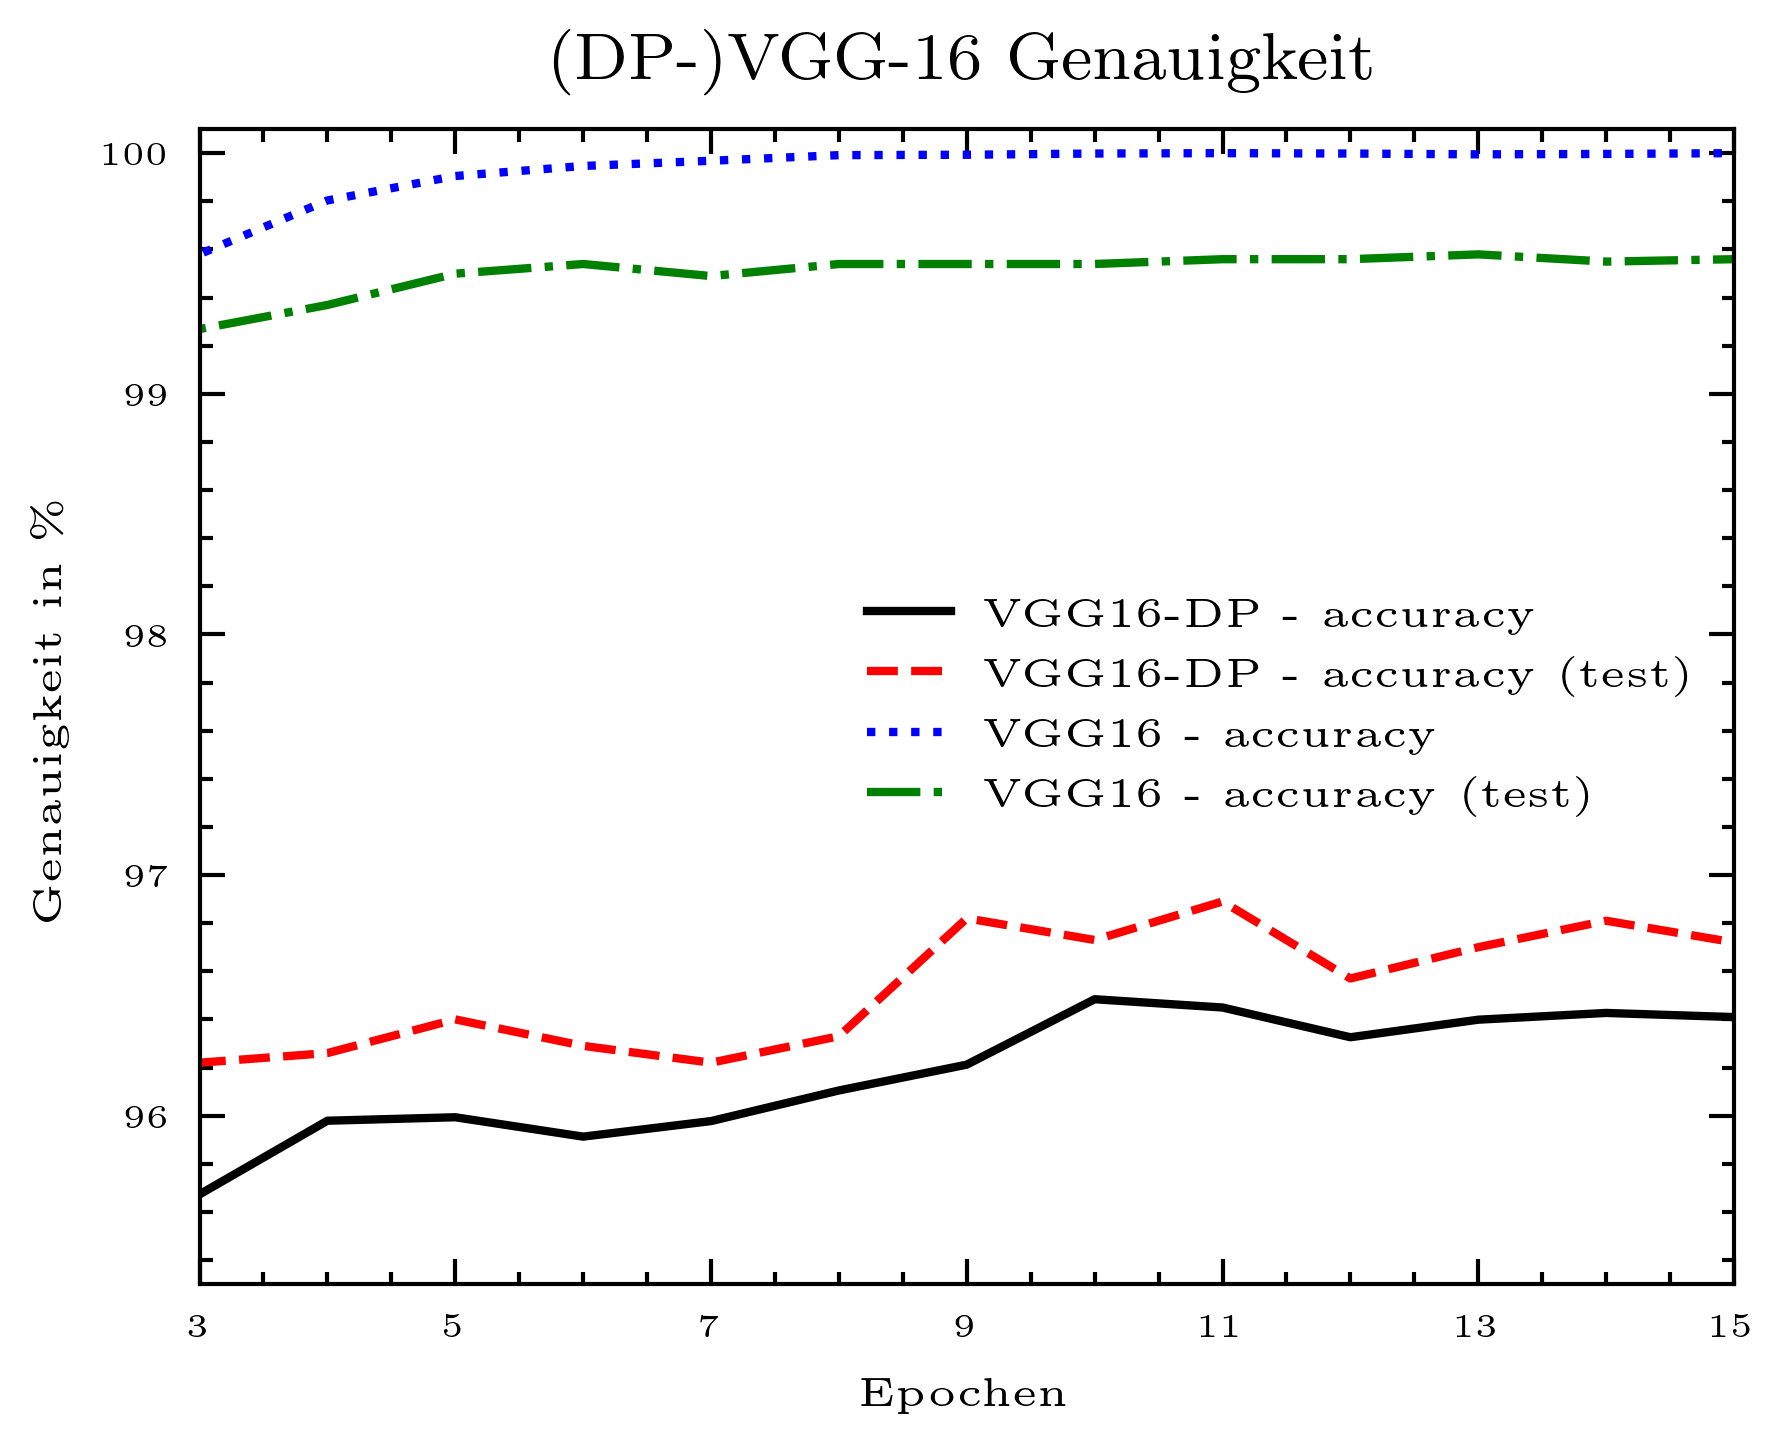
\includegraphics[width=\linewidth, height=4cm]{Bilder/acc.png}
		\caption{Modell-Genauigkeit}
		\label{img:acc_vgg_dp}
	\end{subfigure}
	\hspace{1cm} % Einfügen von horizontalen Abständen zwischen den Bildern
	\begin{subfigure}[b]{0.35\linewidth}
		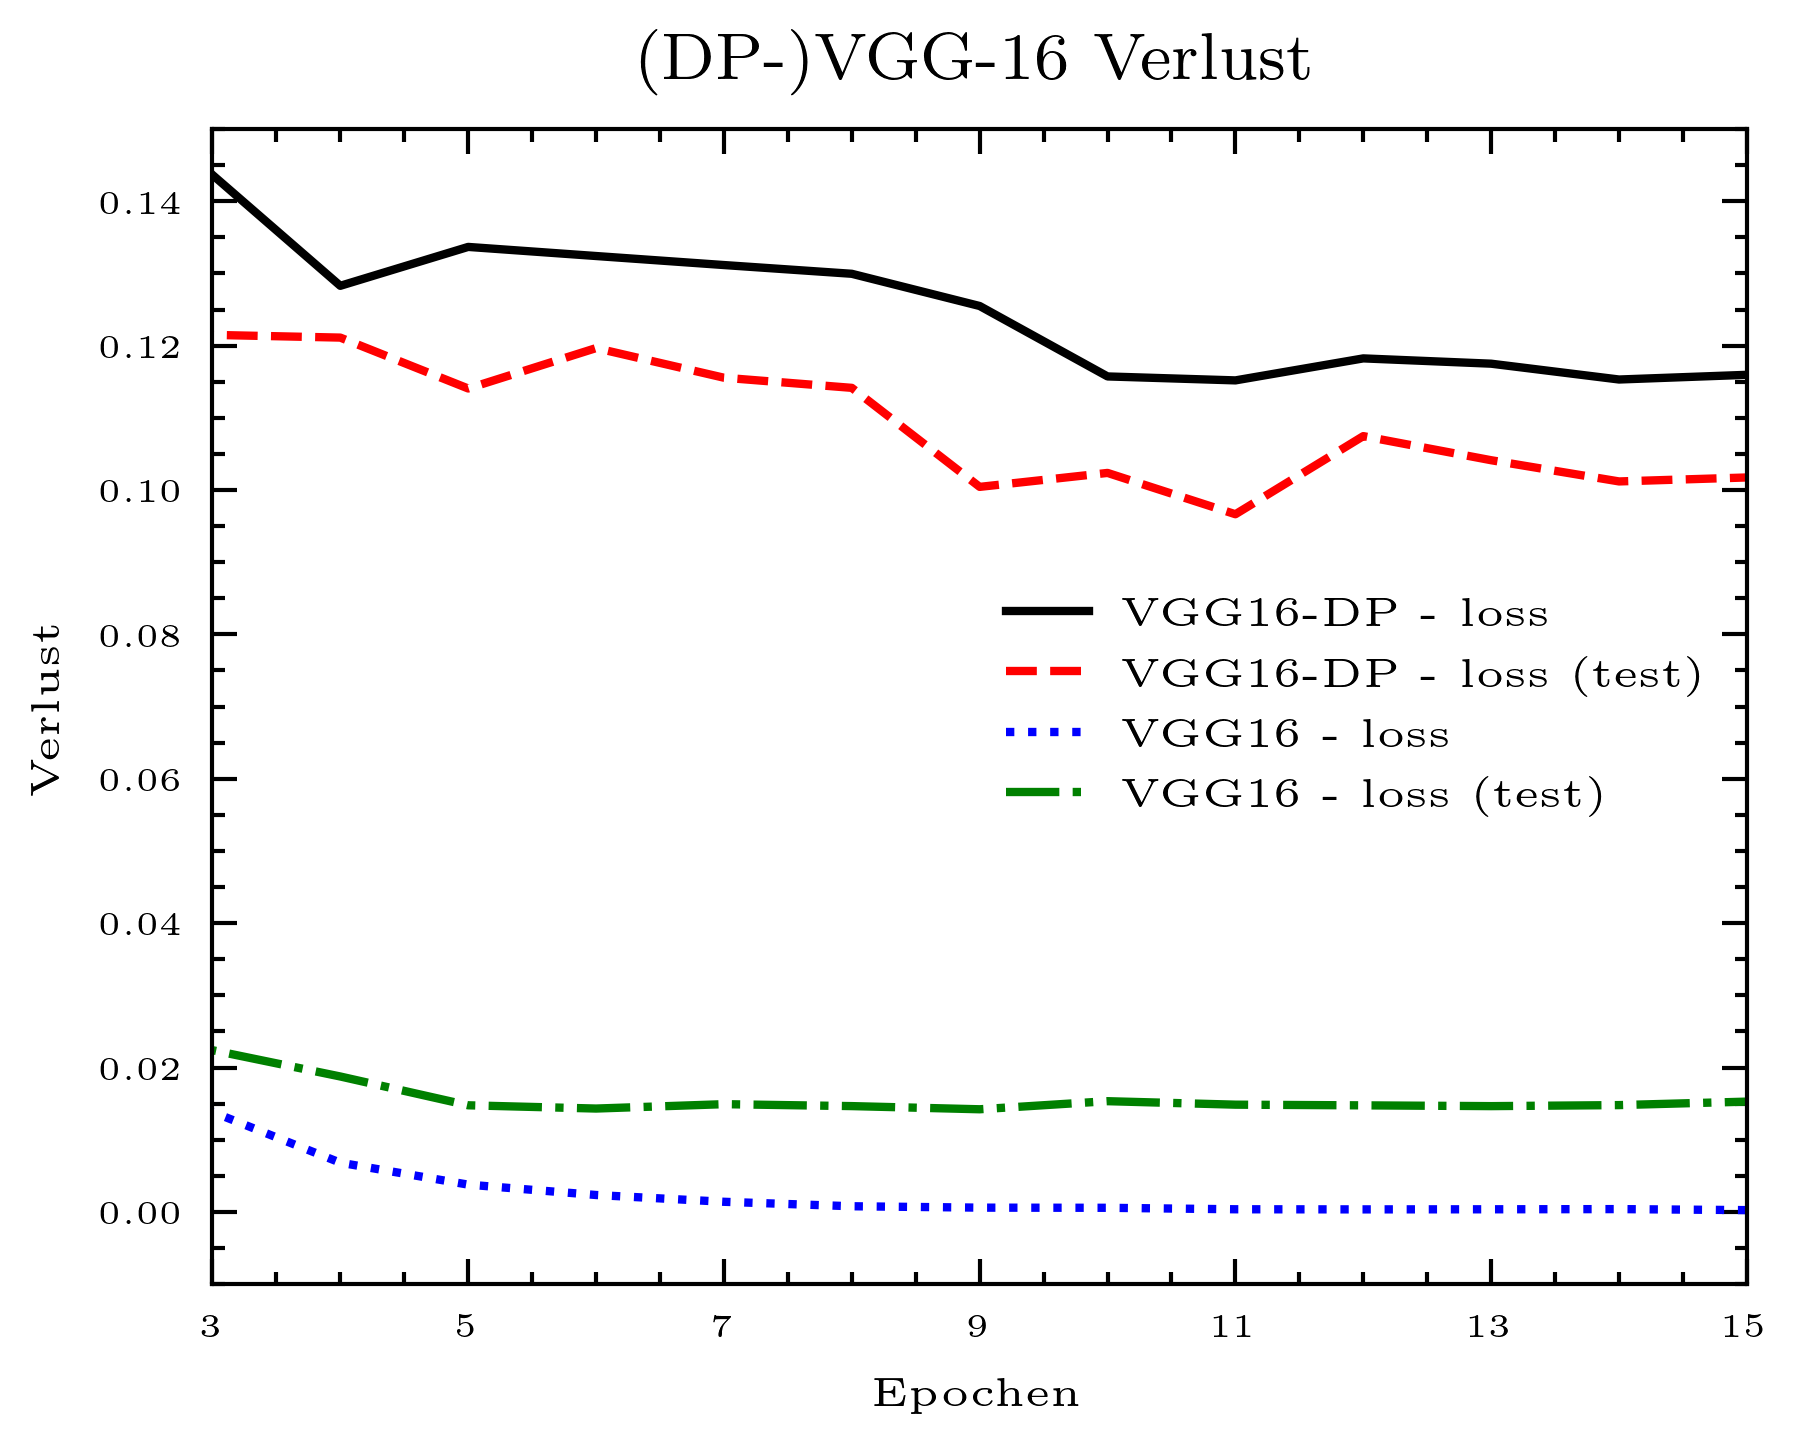
\includegraphics[width=\linewidth, height=4cm]{Bilder/loss.png}
		\caption{Verlust}
		\label{img:loss_vgg_dp}
	\end{subfigure}
	\caption{Verlust- und Genauigkeitsgegenüberstellung eines auf den MNIST-Datensatz normal und privat trainierten Modells}
	\label{img:mnist_figure}
\end{figure}
Die \textit{Genauigkeit} (\(Acc\)) (Bild \ref{img:acc_vgg_dp}) bezüglich der Test- und Trainingsdaten nimmt -- wie erwartet -- im Laufe des Trainingsprozesses zu. 
Diese wird wie folgt definiert: 
\begin{equation}
	Acc = \frac{\text{Anzahl der korrekten Vorhersagen}}{\text{Anzahl der gesamten Vorhersagen}}
\end{equation}
Während das \glqq normale Training\grqq{} mit einer Test-Genauigkeit \(Acc_{\text{test}}\) $\approx99{,}0\%$ startet und bei  \(Acc_{\text{test}}\)$\approx 99{,}5\%$ nach etwa 7 Epochen stagniert, erreicht das \glqq neuronale Netzwerk mit differentieller Privatsphäre\grqq{} zu Beginn einen deutlich niedrigeren Wert von ungefähr $91{,}5\%$ (\(Acc_{\text{test}}\)) und stagniert während der trainierten 15 Epochen noch nicht. Dabei ist allerdings zu Vermuten, dass die Genauigkeit während weiteren Epochen ansteigt, was aufgrund begrenzter Ressourcen nicht getestet werden konnte. Die hohe Genauigkeit des \glqq normalen\grqq{} Modells nach nur einer Trainingsepoche ist auf das Transfer-Learning zurückzuführen, wobei Gewichtungen anhand eines anderen, großen Datensatzes vortrainiert sind, und nicht mit Trainingsstart neu initialisiert werden müssen. 

Der \textit{Verlust} (Bild \ref{img:loss_vgg_dp}) während des Trainings zeigt einen ähnlichen Verlauf wie die oben beschriebene Test-Genauigkeit der beiden Modellarten. Nach etwa 7 Epochen beginnt dieser bei der Durchführung des \glqq normalen Trainings\grqq{} zu konvergieren und deutet darauf hin, dass das Training erfolgreich durchgeführt wurde. Im Gegensatz dazu ist wiederum bei dem \glqq Modell mit differentieller Privatsphäre\grqq{} zu beobachten, dass eine Konvergenz der Verlustfunktion nach 15 Epochen nicht erkannt werden kann. Auch hier -- wie bei Test-Genauigkeit -- lässt sich vermuten, dass eine Erhöhung der Trainingsdurchläufe eine Minimierung der Verlust-Funktion herbeiführt.  Zudem lässt sich bei beiden Modellen aus dem Verlauf der Verlustfunktion ableiten, dass die Modelle keine Überanpassung bezügliche der Trainingsdaten vorweisen. 

Das \glqq normale Training\grqq{} kann aufgrund der konvergierenden Verlust- und Genauigkeitsverte nach 7 Epochen beendet werden, da die Parameter nahezu vollständig an den Datensatz (Bild \ref{img:mnist_figure} - MNIST) angepasst sind. Dahingegen sollte man aufgrund der unvollständigen Parameteranpassung im Modell mit differentieller Privatsphäre die Anzahl der Epochen  erhöhen.

\section{Bildqualität}
Aufgrund der verschiedenen Angriffs-Verfahren variiert die Genauigkeit der Bilder in den unterschiedlichen Durchgängen, wobei die Qualität - abhängig von der Komplexität des Generative-Adversarial Networks - gleich ist. Die Genauigkeit des neu generierten Bildes, das aus privaten Daten abgeleitet ist, wird mit Hilfe des Confidence-Scores bezüglich Ziel-Klasse bestimmt. Im Folgenden werden einige Vergleiche über die Bildqualität nach der Ausführung des Angriffs basierend auf einem Klassifizierungsmodell für Zahlen und Gesichtern aufgezeigt.

Die \textit{Qualität} der Bilder ist abhängig von genutztem GAN (Generative adversarial network), das für die Generierung verwendet wird. Generierungen basierend auf dem DCGAN sind aufgrund geringerer Parameter, kürzerer Trainingsdauer und anderer Faktoren qualitativ nicht so hochwertig wie die des genutzten StyleGANs.

\begin{figure}[H]
	\centering
	\begin{subfigure}[b]{0.35\linewidth}
		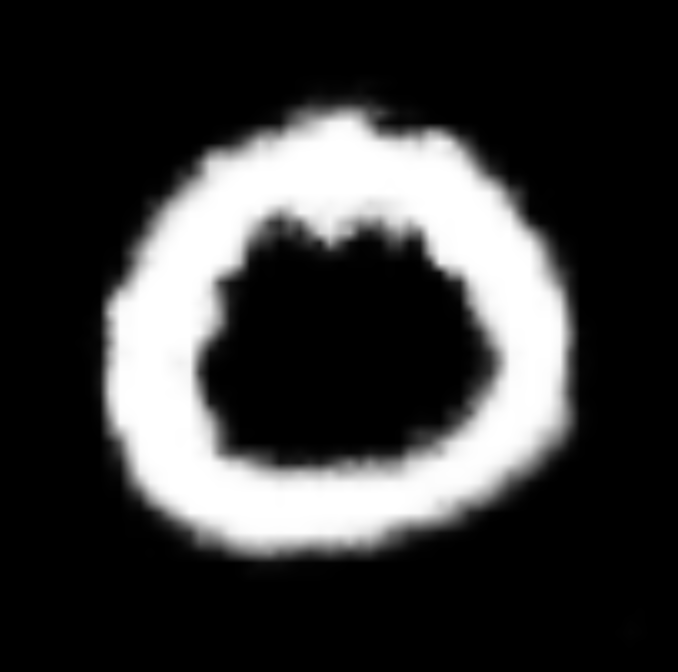
\includegraphics[width=\linewidth]{Bilder/0_mnist.png}
		\caption{Generierung der Zahl 0 auf Basis eines DCGAN}
		\label{img:gen_img_dcgan}
	\end{subfigure}
	\hspace{1cm} % Einfügen von horizontalen Abständen zwischen den Bildern
	\begin{subfigure}[b]{0.35\linewidth}
		
\includegraphics[width=\linewidth]{Bilder/401_celeba.png}
		\caption{Generierung einer Frau mit Hilfe eines StyleGANs}
		\label{img:gen_img_stylegan}
	\end{subfigure}
	\caption{Bildqualität der GAN-Modelle}
	\label{img:gen_img}
\end{figure}
Die Bilder des DCGAN basierten Generators sind etwas schwach mit vergleichsweise wenigen Pixeln aufgelöst (siehe Bild \ref{img:gen_img_dcgan}). Dahingegen lassen sich Bilder des StyleGAN Netzwerks in einer deutlich besseren Auflösung von bis zu 200 $\times$ 200 Pixeln generiern. Wie im Bild \ref{img:gen_img_stylegan} zu erkennen, wird die Qualität der Bilder durch die Reduktion der Pixel deutlich verschlechtert, was aber zu einer effektiveren Angriffsdauer führt. Im Gegensatz zu den generierten Ziffern handelt es sich bei den Gesichtern um 3-Kanal Bilder (RGB), weshalb diese farblich zu betrachtet sind.
\section{Angriffsperformance}
Dieses Kapitel befasst sich mit der Auswertung beider Angriffe nach der Durchführung, wobei im Folgenden ein Vergleich mit dem Ziel der Stärken- und Schwächenbeleuchtung aufgestellt wird. Um die Angriffe besser bewerten zu können, werden zum einen visuelle, aber auch metrische Daten begutachtet, wozu beispielsweise die Genauigkeit der neu generierten Bilder bezüglich der Ziel-Kategorie des \glqq angegriffenen\grqq{} Modells zählt.
\subsection{Genauigkeit der Angriffe}
Um eine präzisere Analyse der Angriffsgenauigkeit zu ermöglichen, werden neben visuellen Metriken auch numerische Kennzahlen integriert, um einen messbaren und vergleichbaren Wert zu erlangen.

Im Zuge der Durchführung eines \glqq KEDMI\grqq-Angriffs auf ein Zielmodell, das für die Klassifikation von handgeschriebenen Ziffern konzipiert ist, wurden entscheidende Erkenntnisse gewonnen, welche die potenzielle Gefahr des Angiffs verdeutlichen und die Notwendigkeit, adäquate Verteidigungsstragegien zu implementieren, unterstreichen. Im Folgenden werden verschiedene Metriken präsentiert, die im Rahmen der Evaluierung Verwendung finden und einen direkten Vergleich zu \glqq RBMI\grqq-Angriffen ermöglichen. Diese bieten Einblicke in die Wirksamkeit, Effektivität und Effizienz der Angriffe sowie die daraus resultierenden Auswirkungn auf die Sicherheits-Komponente des Zielmodells. Die detaillierte Analyse der Evaluierungsmetriken ermöglicht eine Bewertung der durch den Angriff aufkommenden Sschwachstelle. Diese Ergebnisse dienen zudem als Grundlage für die Ableitung geeigneter Schutzmaßnahmen zur Stärkung der Sicherheit und Robustheit des Modells gegenüber Inferenz-Angriffen.

Die visuelle Metrik zur Bewertung der Angriffsqualität stellt einen Vergleich der wiederhergestellten Bilder nach erfolgreicher Durchführung auf ein bestimmtes Zielmodell dar. Dafür werden 60 Bilder aus insgesamt 10 Klassen, die während des Angriffs generiert wurden, mit einer Sammlung von 60 Originalbildern der selben Klasse gegenübergestellt, um diese zu vergleichen. Das Angriffsziel besteht darin, dass Merkmale der Originalbilder visuell mit denen der generierten Bilder übereinstimmen, jedoch nicht jeder einzelne Trainings-Datenpunkt generiert wird.

\begin{figure}[H]
	\centering
	\begin{subfigure}[b]{0.35\linewidth}
		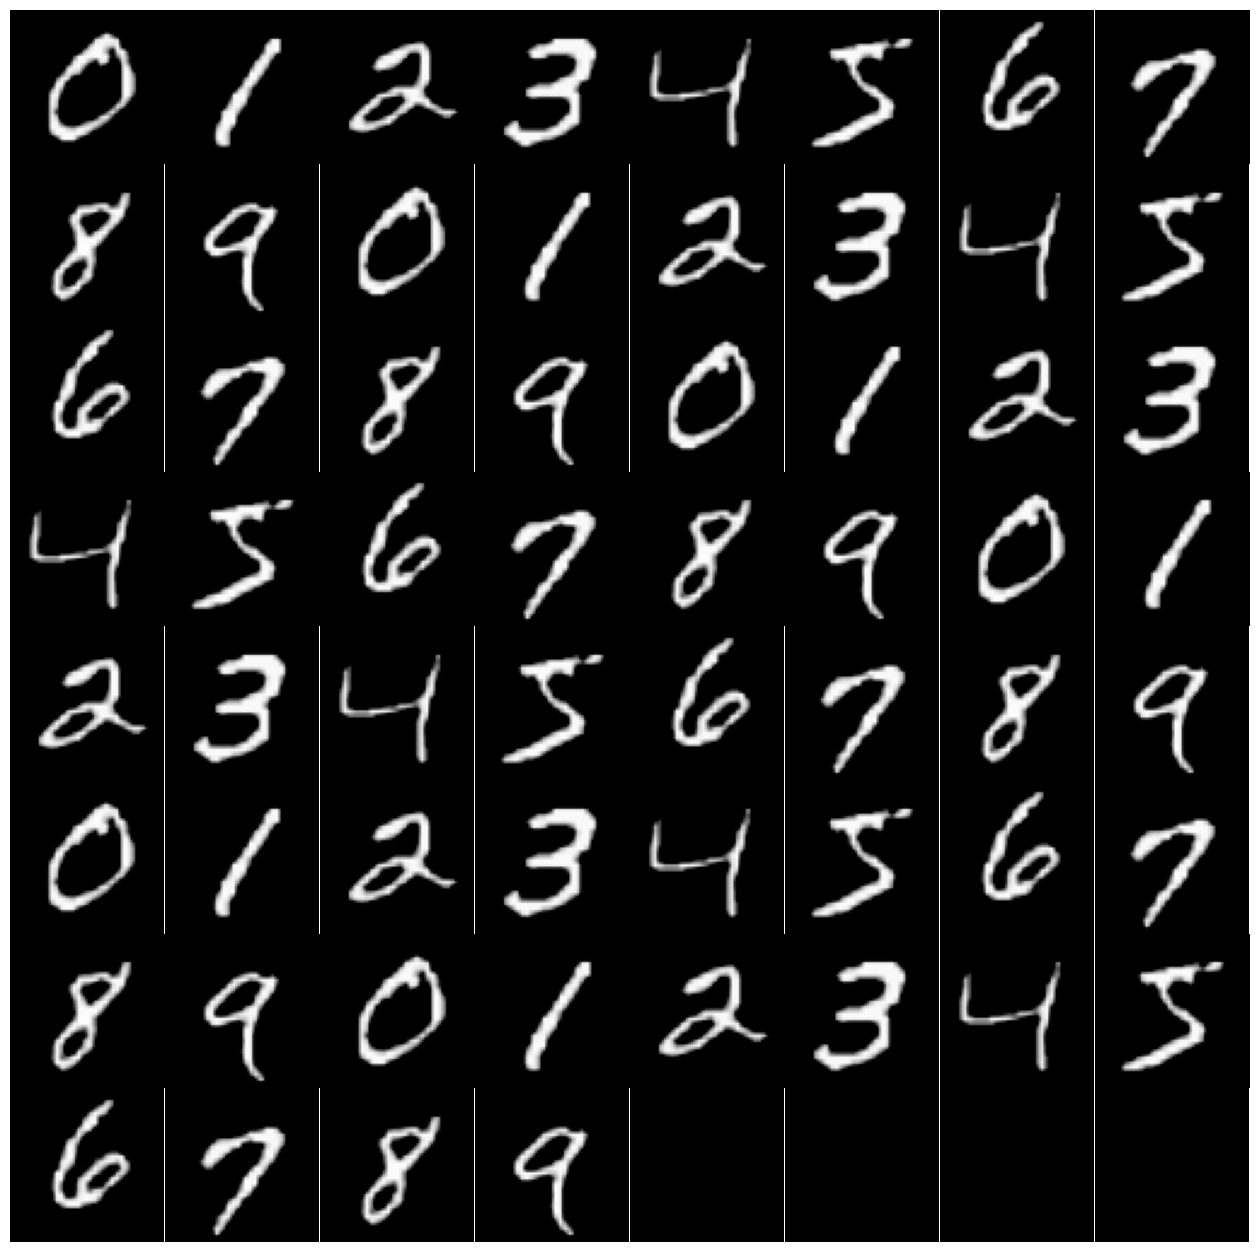
\includegraphics[width=\linewidth]{Bilder/mnist_orig.png}
		\caption{60 Originalbilder des MNIST-Datensatzes}
		\label{img:kedmi_orig}
	\end{subfigure}
	\hspace{1cm} % Einfügen von horizontalen Abständen zwischen den Bildern
	\begin{subfigure}[b]{0.348\linewidth}
		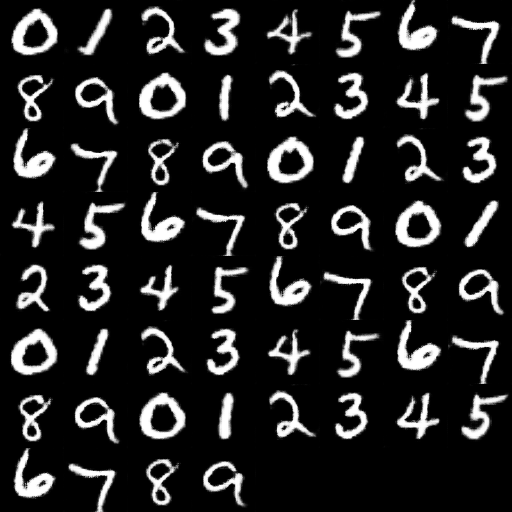
\includegraphics[width=\linewidth]{Bilder/kedmi_mnist.png}
		\caption{60 durch den \glqq KEDMI\grqq-Angriff generierte Bilder}
		\label{img:kedmi_gen}
	\end{subfigure}
	\caption{Gegenüberstellung der generierten und originalen Bilder}
	\label{img:kedmi_visual}
\end{figure}

Es zeigt sich deutlich, dass alle Klassen durch eine konsistente Übereinstimmung zwischen den originalen Bildern (siehe Abbildung \ref{img:kedmi_orig}) des Datensatzes und den generierten Bildern des \textit{"KEDMI"}-Angriffs (siehe Abbildung \ref{img:kedmi_gen}) korrekt wiederhergestellt wurden. Beim Bildvergleich wird ersichtlich, dass die Aufmachung der originalen zu den generierten Bildern variiert, was auf den Trainingsprozess und die Qualität des genutzten Generator-Netzwerks (GAN) zurückzuführen ist. Beispielsweise sind die generierten Ziffern deutlich kräftiger, als die Originalzahlen. Zudem ist erkennbar, dass die Bilder nicht exakt identisch sind, was jedoch nicht das Ziel des Angriffs darstellt, da die Bilder eine durchschnittliche Repräsentation der Features eines bestimmten Labels symbolisieren sollen.

Die visuelle Qualitätsanalyse bezüglich eines weiteren Datensatzes (CelebA) gestaltet sich aufgrund der komplexeren Datenpunktstruktur etwas unklarer im Vergleich zu den auf MNIST basierenen Angriffsgenerierungen. Die Bildqualität des verwendeten Generators (GAN) ist die komplexität der Merkmale signifikant beeinträchtigt. Auch hier werden 60 verschiedene Bilder (je eins pro Kategorie) mit dem jeweiligen Originalen der gleichen Klasse verglichen.

\begin{figure}[H]
	\centering
	\begin{subfigure}[b]{0.35\linewidth}
		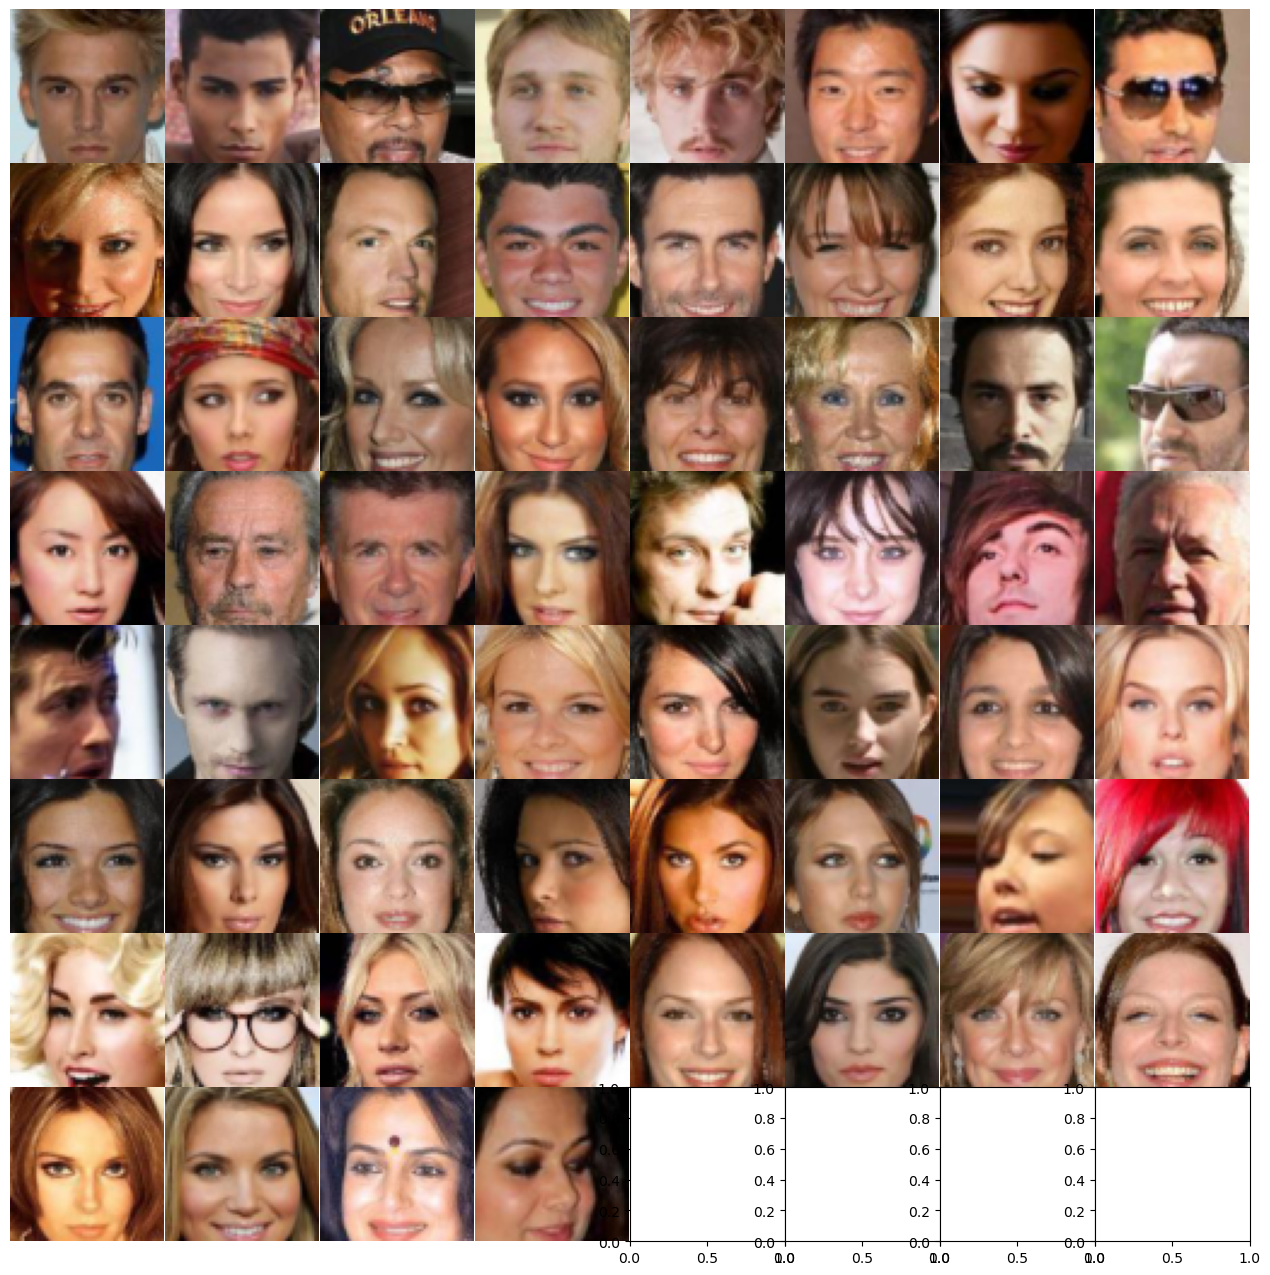
\includegraphics[width=\linewidth]{Bilder/celeba_orig.png}
		\caption{60 Originalbilder des CelebA-Datensatzes}
		\label{img:kedmi_celeba_orig}
	\end{subfigure}
	\hspace{1cm} % Einfügen von horizontalen Abständen zwischen den Bildern
	\begin{subfigure}[b]{0.348\linewidth}
		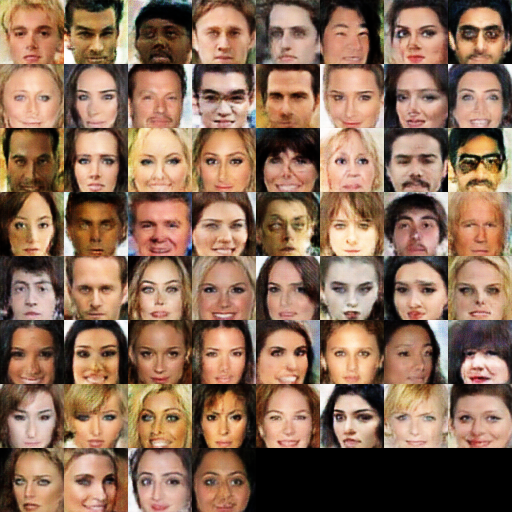
\includegraphics[width=\linewidth]{Bilder/kedmi_celeba.png}
		\caption{60 durch den \glqq KEDMI\grqq-Angriff generierte Bilder}
		\label{img:kedmi_celeba_gen}
	\end{subfigure}
	\caption{Gegenüberstellung der generierten und originalen Bilder}
	\label{img:kedmi_celeba_visuell}
\end{figure}

Bei der Durchführung des \glqq KEDMI\grqq-Angriffs auf einen für Gesichtsdaten trainierten Klassifizierer ist klar erkennbar, dass die zugrundeliegende Person, wenn auch teilweise verzerrt, wiederhergestellt wurde. Die Verzerrung und die daraus resultierende Ungenauigkeit in bestimmten Details sind auf die Bildqualität des generierenden Netzwerks zurückzuführen, das auch bei einfacher Generierung unabhängig von Angriffen Bildfehler einschleust. Es wird ebenfalls deutlich, dass die verschiedenen Bilder nicht vollständig mit dem Original übereinstimmen, da beispielsweise Personen in die \glqq falsche\grqq{} Richtung schauen. Dies ist darauf zurückzuführen, dass der Angriff nicht auf die eindeutige Generierung aller im Training verwendeten Datenpunkte abzielt, sondern auf ein Bild mit maximiertem Confidence-Score bezüglich der Zielklasse, damit dieses vom Klassifizierer mit hoher Sicherheit richtig erkannt wird, um darauf basierend die wichtigsten Features der jeweiligen Klasse symbolisieren zu können. 

Im Gegensatz zu \glqq KEDMI\grqq-Angriffen stellen \glqq RBMI\grqq-Angriffe eine größere Herausforderung bedingt durch die komplexere Angriffsdurchführung dar. 

Mit Hilfe der visuellen Metrik kann auch hier ein Vergleich zwischen generierten und originalen Daten hergestellt werden, um einen Teil der \textit{Angriffsqualität} darstellen zu können. Hierzu werden zehn Originalbilder mit einem durch den Angriff generierten Zielbild verglichen, um eine visuelle Qualitätsschätzung durchführen zu können. Auch hier ist das Ziel des Angriffes, einen \glqq Durchschnittsdatenpunkt\grqq{} zu generieren, der die Features des jeweiligen Ziellabels am besten repräsentiert und somit eine hohe Genauigkeit bezüglich der Zielklasse des Modells hat. 

\begin{figure}[H]
	\centering
	\begin{subfigure}[b]{0.8\linewidth}
		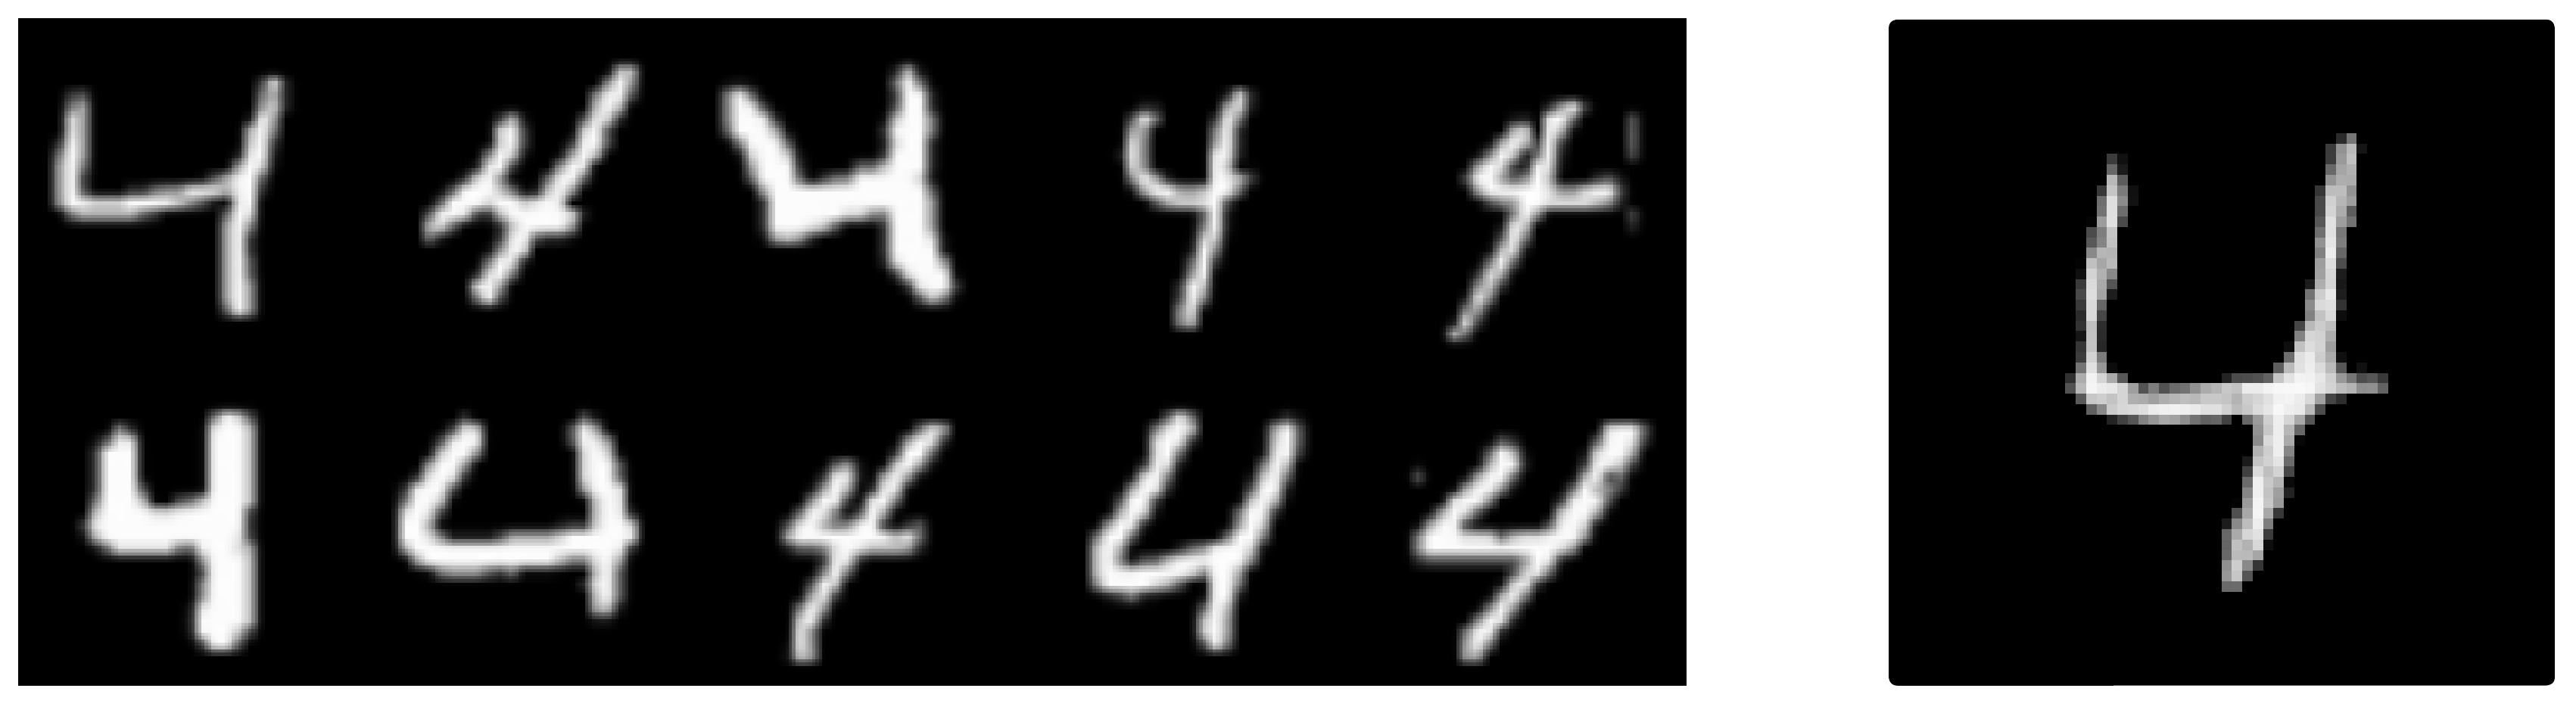
\includegraphics[width=\linewidth, height=5cm, keepaspectratio]{Bilder/4_mnist_rbmi.png}
	\end{subfigure}
	\caption{Gegenüberstellung des generierten Bildes (\textit{rechts}) (mit \glqq RBMI\grqq-Angriff) mit den Originalbildern aus MNIST (\textit{links}) der Zielklasse}
	\label{img:rbmi_visual_mnist}
\end{figure}

Während der Durchführung von Algorithmen zur Rückgewinnung von Trainingsdaten fällt auf, dass der black-box-basierte \glqq RBMI\grqq-Angriff Bilder generiert, die in jeder Klasse visuell korrekte Darstellungen hervorbringen. Diese Beobachtung basiert auf einem Vergleich zwischen den generierten und den originalen Bildern (aus Abbildung \ref{img:rbmi_visual_mnist}). Deutlich erkennbar ist, dass die zurückgewonnenen Bilder mit den Originalbildern in Übereinstimmung stehen. Diese Übereinstimmung manifestiert sich in einer hohen \textit{visuellen Angriffsqualität}, die mit jener des \glqq KEDMI\grqq-Angriffs vergleichbar ist.

\begin{figure}[H]
	\centering
	\begin{subfigure}[b]{0.8\linewidth}
		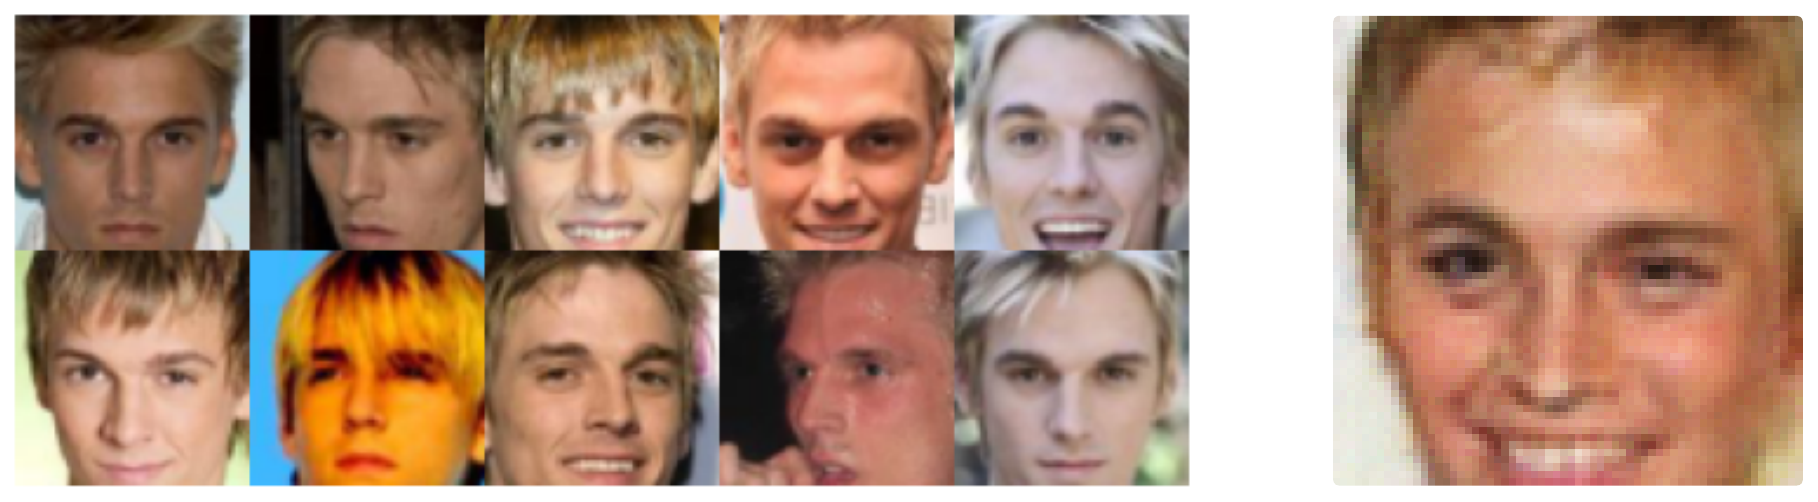
\includegraphics[width=\linewidth, height=5cm, keepaspectratio]{Bilder/0_celeba_rbmi.png}
	\end{subfigure}
	\caption{Gegenüberstellung des generierten Bildes (\textit{rechts}) (mit \glqq RBMI\grqq-Angriff und DCGAN) mit den Originalbildern aus CelebA (\textit{links}) der Zielklasse}
	\label{img:rbmi_visual}
\end{figure}

Für die Angriffsvalidierung werden auch hier (Abbildung \ref{img:rbmi_visual}) Originalbilder mit Generierungen basierend auf den CelebA-Datensatz verglichen. Das rechte Bild wurde durch die Ausführung eines \glqq RBMI\grqq-Angriffs unter Verwendung des DCGAN-Generators generiert. Die Qualität der erzeugten Bilder ist unmittelbar mit der Generierungsfähigkeit des Generators verbunden. Da der Generator lediglich Bilder mit einer Größe von 64 $\times$ 64 Pixeln erstellen kann, bleibt die Auflösung der rückgenerierten Bilder entsprechend begrenzt. Deutlich zu erkennen ist allerdings, dass das generierte Bild mehrere Features aus den verschiedenen Trainingsbildern darstellt und dadurch auf eine positive Angriffsdurchführung hindeutet.

\begin{figure}[H]
	\centering
	\begin{subfigure}[b]{0.8\linewidth}
		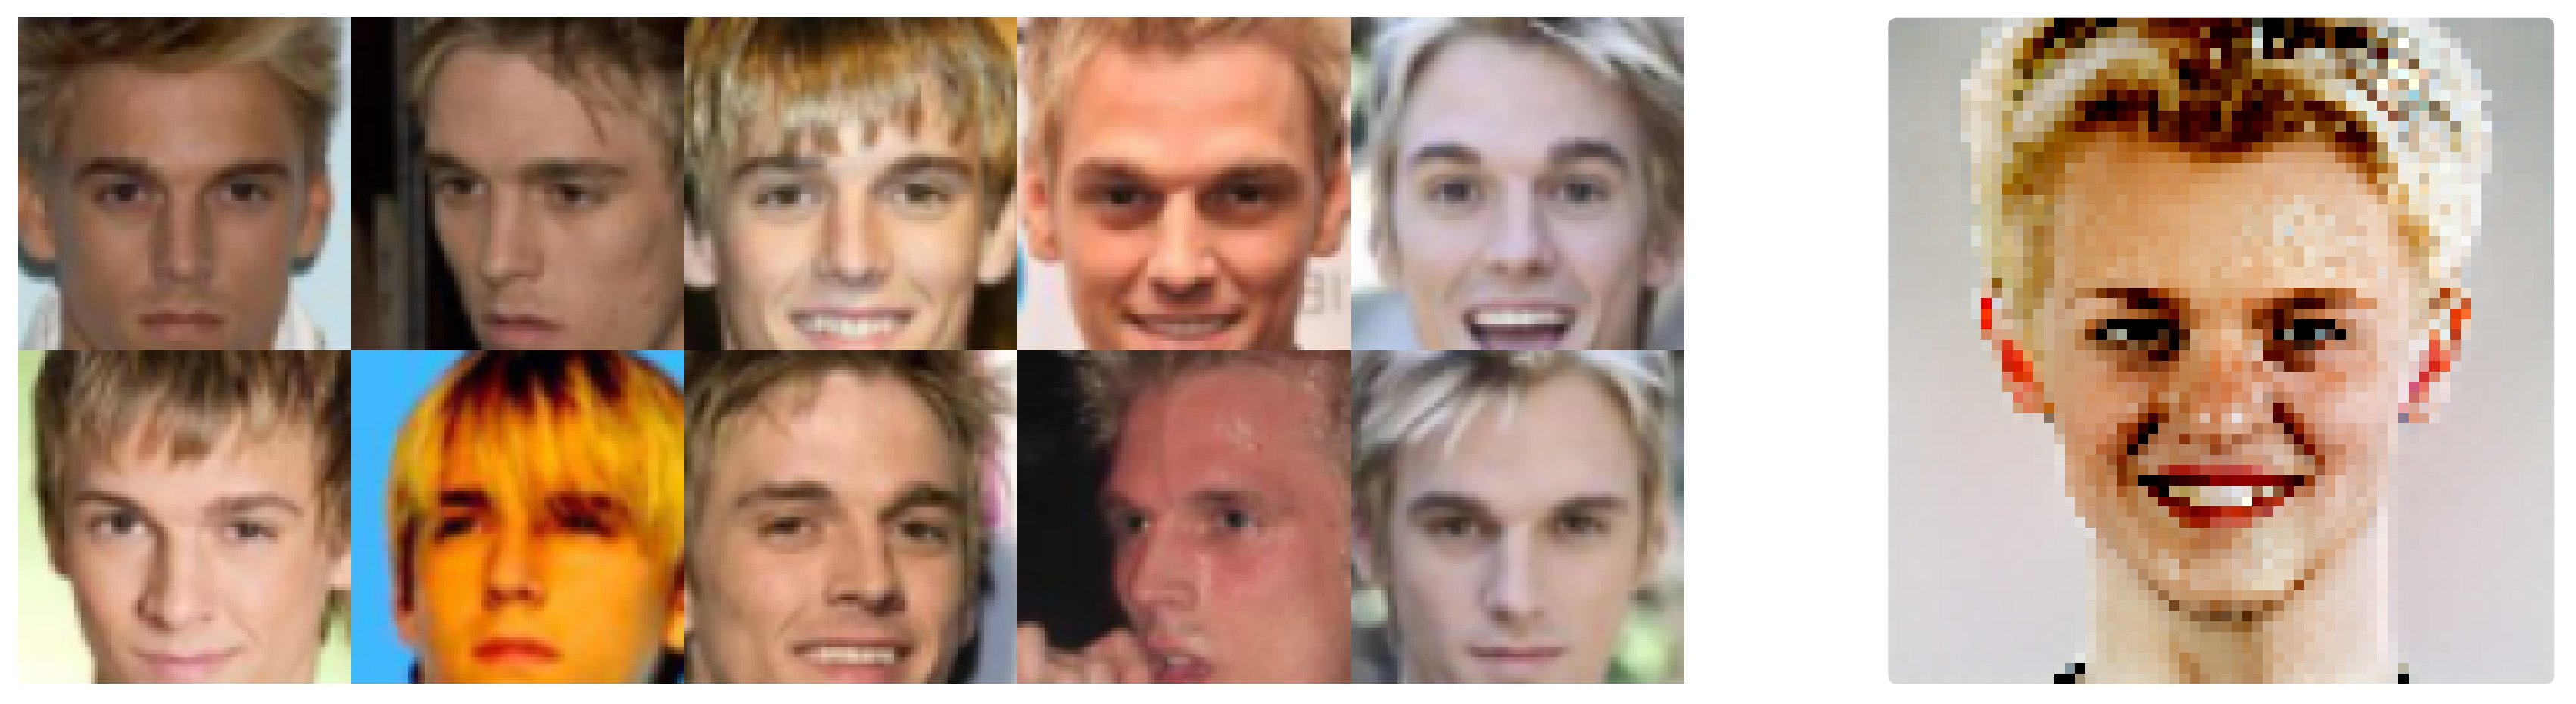
\includegraphics[width=\linewidth, height=5cm, keepaspectratio]{Bilder/0_celeba_rbmi_stylegan.png}
	\end{subfigure}
	\caption{Gegenüberstellung des generierten Bildes (\textit{rechts}) (mit \glqq RBMI\grqq-Angriff und StyleGAN) mit den Originalbildern aus CelebA (\textit{links}) der Zielklasse}
	\label{img:rbmi_visual_stylegan}
\end{figure}

Um die \textit{Qualität} des Angriffs auf visueller und statistischer Ebene eingehender zu analysieren, wurde ein Generator basierend auf der Style-GAN-Architektur verwendet, der auf einem unabhängigen Datensatz trainiert ist (\cite{noauthor_nvlabsffhq-dataset_2023}). Dieser Ansatz ermöglicht eine umfassendere Bewertung der erzeugten Bilder, wobei visuelle und statistische Merkmale gleichermaßen berücksichtigt werden.

Die Abbildung \ref{img:rbmi_visual_stylegan} illustriert, dass der Generationsprozess mittels des Style-GAN-Generators zu Bildern führt, die die repräsentativen Merkmale der Originalperson aufweisen. Beispiele hierfür sind unter anderem die blonden Haare und andere charakteristische Eigenschaften wie Ohren. Es ist anzumerken, dass das neu generierte Gesicht eine höhere Auflösung aufweist, die aufgrund der besseren Qualität des Generators erzielt wird. Während des Algorithmus wird diese Auflösung jedoch auf 64 $\times$ 64 Pixel reduziert, um eine effiziente Ausführung zu gewährleisten.

Bei genauerer Betrachtung wird ersichtlich, dass das generierte Bild Features aus mehreren Trainingsbildern integriert. Diese Vorgehensweise zielt darauf ab, eine möglichst hohe Genauigkeit bezüglich der Zielklasse zu erreichen. Insbesondere werden Merkmale, die in verschiedenen Trainingsbeispielen präsent sind, kombiniert, um eine umfassende Repräsentation der Zielklasse zu gewährleisten.

Die hohe Auflösung des generierten Gesichts, kombiniert mit der Integration von Merkmalen aus mehreren Trainingsbildern, verdeutlicht die anspruchsvolle Generierung von Bildern durch den \glqq RBMI\grqq-Angriff unter Verwendung des Style-GAN-Generators. Dieser Ansatz zeugt von einer verbesserten visuellen Qualität und statistischen Relevanz im Vergleich zu einfachen Generatoren, was die Notwendigkeit betont, solche fortgeschrittenen Techniken bei der Entwicklung von Verteidigungsstrategien gegen Modellinversionsangriffe zu berücksichtigen.

Die visuelle Angriffsqualität wird dabei als Kriterium herangezogen, um die visuelle Ähnlichkeit zwischen den generierten und den originalen Bildern zu bewerten. Diese Qualität ist bei dem \glqq RBMI\grqq-Angriff als hoch einzustufen, was darauf hinweist, dass die rückgewonnenen Bilder die visuellen Merkmale und Strukturen der Originalbilder präzise wiedergeben. Dieses Phänomen findet Analogie zu der Beobachtung, die bereits beim \glqq KEDMI\grqq-Angriff festgestellt wurde.

Die visuelle Übereinstimmung zwischen generierten und originalen Bildern ist ein entscheidendes Kriterium für die Wirksamkeit von Modellinversionsangriffen, insbesondere im Hinblick auf die Erhaltung von Klassenmerkmalen und Strukturdetails. Die hohe visuelle Angriffsqualität beider Algorithmen deutet darauf hin, dass diese Ansätze eine erfolgreiche Rückgewinnung von Trainingsdaten ermöglichen und somit potenzielle Risiken für die Sicherheit und Vertraulichkeit von Modellen darstellen.
\subsection{Angriffsstatistiken}
%KEDMI
Um über visuelle Qualitätsmerkmale hinaus zusätzliche Metiken einführen zu können, werden im Folgenden detaillierte Vergleiche durch verschiedene statistische Analysen mit dem Ziel des Angriffvergleichs und der Auflistung von Leistungsfähigkeiten präsentiert. Besondere Aufmerksamkeit wird dabei auf die Angriffsdauer und die Genauigkeit der Angriffe gelegt. Durch die Anwendung statistischer Methoden wird ein systematischer Vergleich der Angriffsleistungen ermöglicht, wobei eine Analyse dieser statistischen Parameter eine Rückschlussziehung bezüglich der Leistungsfähigkeit der Angriffe bietet.

Des Weiteren wird die Genauigkeit der Angriffe als entscheidende Metrik betrachtet. Dadurch soll die visuelle Einstimmigkeit zwischen Generierung und Originalbild belegt werden, indem man Kennzahlen über die Genauigkeit der Vorhersage des Zielmodells interpretiert. Diese Erkenntnisse tragen dazu bei, die Wirksamkeit der Angriffe in verschiedenen Kontexten zu bewerten und möglicherweise Optimierungspotenziale zu identifizieren.

\begin{table}[h]
	\centering
	\renewcommand{\arraystretch}{1.5}
	\resizebox{\textwidth}{!}{
		\begin{tabular}{|c|c|c|c|c|c|c|}
			\hline
			\textbf{Modell-Art} & \textbf{Generator} & \textbf{Datensatz} & \textbf{Iterationen} & \textbf{Dauer pro Iteration} & \textbf{Gesamtdauer} & \textbf{Genauigkeit}\\
			\hline
			\textit{VGG-16} & DCGAN & MNIST & 2.400 & 0,11 sec & 4 min & \textbf{100,0\%}\\
			\hline
			\textit{VGG-16} & DCGAN & CelebA & 2.400 & 0,12 sec & 4 min & \textbf{100,0\%}\\
			\hline
		\end{tabular}
	}
	\caption{\glqq KEDMI\grqq-Angriffsstatistik}
	\label{tab:kedmi_stats}
\end{table}

Die Tabelle \ref{tab:kedmi_stats} präsentiert einen detaillierten Vergleich hinsichtlich der Ausführung des \glqq KEDMI\grqq-Angriffs zwischen dem MNIST- und dem CelebA-Datensatz. Die Resultate verdeutlichen, dass die zeitliche Komponente der Angriffe lediglich um wenige Millisekunden pro Iteration varriert, was auf die Anwendung desselben Algorithmus, identischer Bildgröße und einer gleichbleibenden GAN-Architektur zurückzuführen ist. In diesem Zusammenhang wurden vordefinierte 2000 Iterationen pro Rückgenerierung verwendet, um eine maximal mögliche Genauigkeit zu gewährleisten. Diese erreicht bei beiden Angriffen einen Wert von 100\%, was auf eine korrekte Klassifikation der generierten Bilder durch das Zielmodell hindeutet. 

Die 100\%ige Genauigkeit erstreckt sich über die Rückgewinnung von vergleichsweise simplen Datenpunkten aus dem MNIST-Datensatz bis hin zu Datenpunkten mit komplexeren Merkmalen, wie beispielsweise Gesichtsbildern des CelebA-Datensatzes. Dies bezeugt die Robustheit und Wirksamkeit des \glqq KEDMI\grqq-Angriffs über verschiedene Datensätze und verdeutlicht die Fähigkeit des Algorithmus, eine akkurate Bildqualität und Übereinstimmung zwischen Generierung und Original, unabhängig von der Datenkomplexität, sicherzustellen.

Die Konsistenz der Genauigkeit in verschiedenen Kontexten unterstreicht die Zuverlässigkeit des \glqq KEDMI\grqq-Angriffs und legt nahe, dass dieser Ansatz auch in komplexeren Szenarien anwendbar ist. Diese Erkenntnisse ermöglichen nicht nur eine tiefgehende Bewertung der Angriffsleistung, sondern bieten auch Einblicke in die Generalisierungsfähigkeiten über unterschiedliche Datensätze und Merkmalskomplexitäten hinweg.
%RBMI
\begin{table}[h]
	\centering
	\renewcommand{\arraystretch}{1.5}
	\resizebox{\textwidth}{!}{
		\begin{tabular}{|c|c|c|c|c|c|c|}
			\hline
			\textbf{Modell-Art} & \textbf{Generator} & \textbf{Datensatz} & \textbf{Iterationen} & \textbf{Dauer pro Iteration} & \textbf{Gesamtdauer} & \textbf{Genauigkeit}\\
			\hline
			\textit{VGG-16} & DCGAN & MNIST & 40.000 & 0,018 sec & 12 min & \textbf{100,0\%}\\
			\hline
			\textit{VGG-16} & DCGAN & CelebA & 40.000 & 0,024 sec & 16 min & \textbf{99,94\%}\\
			\hline
			\textit{VGG-16} & StyleGAN & CelebA & 100.000 & 0,085 sec & 142 min & \textbf{98,44\%}\\
			\hline
		\end{tabular}
	}
	\caption{\glqq RBMI\grqq-Angriffsstatistik}
	\label{tab:rbmi_stats}
\end{table}

Die Tabelle \ref{tab:rbmi_stats} verdeutlicht die Angriffsstatistik des \glqq RBMI\grqq-Angriffs. Auch dieser Angriff wurde in verschiedenen Szenarien auf seine Wirksamkeit hin getestet, und die Ergebnisse werden in Form von Metriken dokumentiert. Die Untersuchung zeigt, dass der \glqq RBMI\grqq-Angriff in verschiedenen Kontexten konsistente und überzeugende Ergebnisse liefert. Die Metriken spiegeln die Effektivität des Angriffs wider und bieten Einblicke in seine Leistungsfähigkeit auf Basis unterschiedlicher Bedingungen. Während des Angriffs wurden verschiedene Testläufe durchgeführt, wobei sowohl einfache als auch komplexe Datenpunkte berücksichtigt wurden. Zusätzlich zu den in der \glqq KEDMI\grqq-Statistik (Tabelle \ref{tab:kedmi_stats}) befindlichen Angriffen wurde hier auch ein weiteres Szenario getestet. Dieses umfasst einen Angriff ohne das Kennen des eigentlichen Datensatzes. Dabei wurde ein Generator verwendet, der auf Basis des FFHQ-Datensatzes (\cite{noauthor_nvlabsffhq-dataset_2023})  trainiert ist. 

Die erzielten Ergebnisse weisen darauf hin, dass der \glqq RBMI\grqq-Angriff in der Lage ist, genaue Klassifikationen zu erreichen, unabhängig von der Komplexität der betrachteten Daten. Dies belegt die Robustheit und Anpassungsfähigkeit des Angriffsalgorithmus an verschiedene Datensätze. Insbesondere wurden Metriken verwendet, um den Fortschritt und die Genauigkeit des Angriffs zu quantifizieren. Die erzielten Ergebnisse verdeutlichen, dass der \glqq RBMI\grqq-Angriff nicht nur in der Lage ist, sich an unterschiedliche Datensätze anzupassen, sondern auch eine konstante und zuverlässige Leistung in verschiedenen Szenarien aufweist. Hervorzuheben ist hierbei, dass auf Basis eines komplexen Generators (StyleGAN), der mit vom Zielmodell unabhängen Daten trainiert ist, ein sehr hohe Genauigkeit in Betracht auf die Zielklasse erreicht wurde, ohne dabei Parameter des Modells zu kennen.

Um einen Vergleich zwischen den beiden Angriffsmethoden, KEDMI und RBMI, anzustellen, werden sowohl die Dauer des Angriffs als auch die Genauigkeit betrachtet. Die Analyse der Angriffsqualität legt nahe, dass beide Methoden in der Lage sind, hochwertige Generierungen basierend auf den zugrunde liegenden Trainingsdaten zu erstellen, wobei unterschiedliche Algorithmen zum Einsatz kommen. Der KEDMI-Angriff weist lediglich den Nachteil auf, dass er auf Whitebox-Prinzipien basiert und somit Zugang zu Modellparametern und Trainingsdaten erfordert. Im Gegensatz dazu ist der RBMI-Angriff blackbox-basiert und kann auf jedes Modell angewendet werden, dessen Outputklassen bekannt sind und ein ähnlicher Datensatz vorhanden ist. Ein Nachteil des RBMI-Angriffs besteht jedoch in der Dauer, da dieser einerseits mehr Zeit pro Iteration beansprucht und andererseits eine deutlich höhere Anzahl von Iterationen erfordert.

In qualitativer Hinsicht zeigen beide Angriffe Ähnlichkeiten. Die Güte des Ergebnisses korreliert positiv mit der Bildqualität des Generators. Allerdings verlängert sich die Dauer des RBMI-Angriffs mit zunehmender Bildqualität, wie aus der letzten Zeile der Tabelle \ref{tab:rbmi_stats} hervorgeht. In diesem speziellen Fall wurde eine Genauigkeit von über 98\% erst nach 100.000 Iterationen erreicht, was der Durchführung des Angriffalgorithmus geschuldet ist. Es ist anzumerken, dass die höhere Iterationsanzahl zu einer verbesserten Genauigkeit führt, jedoch auch die Gesamtdauer des Angriffs erheblich verlängert.
% Genauigkeit normal
% Dauer
\section{Auswertung der Verteidigungsstrategie}\label{chpt:dpnn_stats}
% Genauigkeit dp
Das folgende Unterkapitel widmet sich der umfassenden Auswertung der Verteidigungsstrategie "Differential Privacy". Ziel ist es, die Sinnhaftigkeit dieser Strategie zu bewerten und insbesondere zu untersuchen, wie sich die Integration von Differential Privacy während des Trainingsprozess auf die Genauigkeit von Angriffen auswirkt. Differential Privacy ist eine vielversprechende Methode zum Schutz von Datenschutz und Sicherheit in maschinellen Lernmodellen. Hier werden verschiedene Aspekte analysiert, darunter die Effektivität der Differential Privacy in der Verteidigung gegenüber Angriffen sowie mögliche Auswirkungen auf die Genauigkeit von Angriffen und Klassifikationen. Die Untersuchung berücksichtigt sowohl quantitative Metriken als auch qualitative Aspekte, um ein umfassendes Bild der Wirksamkeit dieser Verteidigungsstrategie zu erhalten. Ziel ist es, zu bewerten, inwieweit Differential Privacy als sinnvoller Schutzmechanismus für maschinelle Lernmodelle fungiert und welche Auswirkungen dies auf die Präzision von Angriffen und Klassifikationen hat.

\begin{figure}[H]
	\centering
	\begin{subfigure}[b]{0.35\linewidth}
		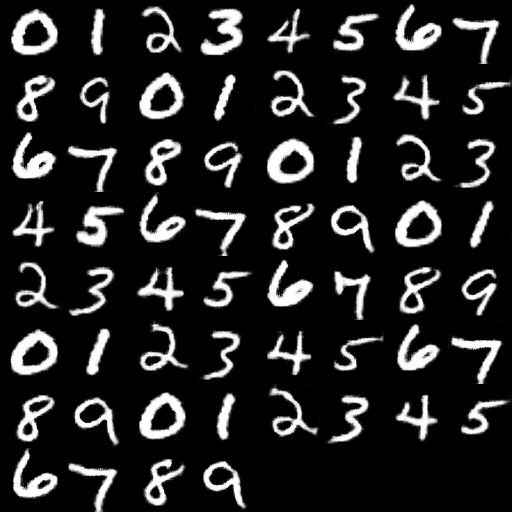
\includegraphics[width=\linewidth]{Bilder/mnist_kedmi.png}
		\caption{Generierung auf Basis eines normalen Modells}
		\label{img:kedmi_mnist}
	\end{subfigure}
	\hspace{1cm} % Einfügen von horizontalen Abständen zwischen den Bildern
	\begin{subfigure}[b]{0.35\linewidth}
		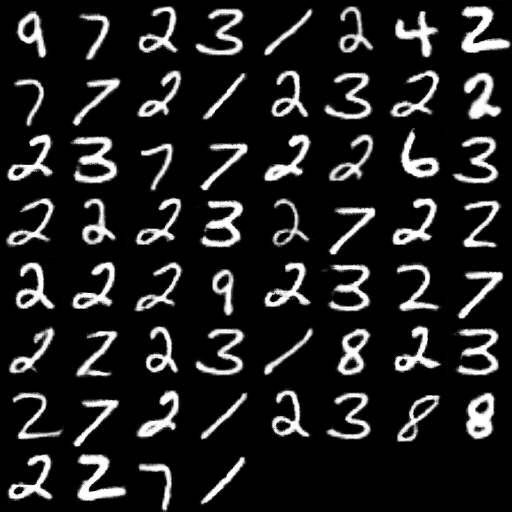
\includegraphics[width=\linewidth]{Bilder/mnist_kedmi_dp.png}
		\caption{Generierung auf Basis eines DP-Modells}
		\label{img:kedmi_mnist_dp}
	\end{subfigure}
	\caption{Gegenüberstellung von Rückgenerierungen basierend auf einem normalen Klassifizierer und einem mit differentieller Privatsphäre mit Hilfe des \glqq KEDMI\grqq-Angriffs}
	\label{img:kedmi_dpvsnorm}
\end{figure}

Im vorliegenden Experiment wurden insgesamt 120 Bilder erzeugt, wobei für jede der zehn Klassen des MNIST-Datensatzes jeweils 6 Bilder verwendet wurden. Die Generierung erfolgte mithilfe einer Modellinversionsattacke, die auf einem herkömmlichen VGG16-Netzwerk basierte. Eine Gruppe von 60 Bildern wurde auf Basis des normalen VGG16-Modells generiert (Beispiel siehe Bild \ref{img:kedmi_mnist}), während die restlichen 60 Bilder unter Verwendung eines VGG16-Modells erstellt wurden, das unter Anwendung differenzieller Privatsphäre trainiert wurde (Beispiel siehe Bild \ref{img:kedmi_mnist_dp}). Die visuelle Analyse dieser umfangreichen Bildersammlung ermöglicht interessante Einblicke in die Wirksamkeit und Robustheit der jeweiligen Modelle.

Die Betrachtung der Bilder, die auf dem konventionellen VGG16-Modell basieren, wie beispielhaft in Bild \ref{img:kedmi_mnist} dargestellt, offenbart eine erfolgreiche Generierung für jede der zehn Zielklassen des MNIST-Datensatzes. Die präzisen Darstellungen spiegeln die Intention des Angriffs wider, die einzelnen Ziffern akkurat zu reproduzieren. Dieses Ergebnis unterstreicht die Fähigkeit des Angriffs, aus dem konventionellen Modell die gewünschten Muster und Merkmale adäquat zu rekonstruieren.

Hingegen zeigt die Betrachtung der Bilder, die auf dem VGG16-Modell mit differenzieller Privatsphäre basieren, wie in Bild \ref{img:kedmi_mnist_dp} exemplarisch dargestellt, auffällige Abweichungen. Die Generierung der Zielklassen weicht zumeist erheblich von der beabsichtigten Darstellung ab, und stattdessen scheinen andere Ziffern in der visuellen Ausgabe präsent zu sein. Diese Unstimmigkeit in der Generierung kann auf die Implementierung differenzieller Privatsphäre zurückgeführt werden, die dem Modell durch ein Rauschen in den Trainingsdaten einen Schutz hinzufügt, um die Vertraulichkeit zu gewährleisten.

Die festgestellte Abweichung zwischen den beiden Gruppen von Bildern belegt, dass die visuelle Repräsentation der Zielklassen durch das Modell mit differenzieller Privatsphäre effektiv verfremdet wurde. Dies lässt darauf schließen, dass die Verteidigungsstrategie in Form der Integration differenzieller Privatsphäre erfolgreich greift. Die Verfälschung der visuellen Ausgabe verhindert, dass sensible Informationen aus den Trainingsdaten extrahiert werden können.

Eine mögliche Erklärung für die fehlgeschlagene KEDMI-Ausführung auf das Zielmodell mit differenzieller Privatsphäre liegt in der Natur des Angriffs selbst. KEDMI ist ein Whitebox-Angriff, der darauf abzielt, interne Merkmale des Modells zu extrahieren. Da der Angriff bei der differentialen Privatsphäre auf ein Rauschen in den Trainingsdaten stößt, wird die Extraktion genauer Merkmale erschwert. Das Fehlschlagen des Angriffs deutet darauf hin, dass das Modell mit differenzieller Privatsphäre nicht nur einen effektiven Schutz für individuelle Daten bietet, sondern auch erfolgreich gegenüber Whitebox-MI-Angriffen widerstandsfähig ist. Diese Resistenz gegenüber KEDMI legt nahe, dass das Modell ohne Overfitting trainiert wurde und somit keine sensiblen Informationen durch gezielte Angriffe extrahiert werden können.

\begin{figure}[H]
	\centering
	\begin{subfigure}[b]{0.35\linewidth}
		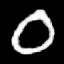
\includegraphics[width=\linewidth]{Bilder/0_rbmi.png}
		\caption{Generierung der Zahl 0 eines normalen Modells}
		\label{img:rbmi_0}
	\end{subfigure}
	\hspace{1cm} % Einfügen von horizontalen Abständen zwischen den Bildern
	\begin{subfigure}[b]{0.35\linewidth}
		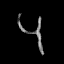
\includegraphics[width=\linewidth]{Bilder/0_rbmi_dp.png}
		\caption{Generierung der Zahl 0 eines DP-Modells}
		\label{img:rbmi_0_dp}
	\end{subfigure}
	\caption{Gegenüberstellung von Rückgenerierungen der Zahl 0 basierend auf einen normalen Klassifizierer und einem mit differentieller Privatsphäre mit Hilfe des \glqq RBMI\grqq-Angriffs}
	\label{img:rbmi_dpvsnorm}
\end{figure}

In einem weiteren Test wurde die Wirksamkeit der Modelle in Bezug auf eine alternative Modellinversionsattacke, nämlich die RBMI Methode, evaluiert. Hierbei wurden 2 Bilder generiert, wobei die Zielsetzung darin bestand, die Repräsentationsfähigkeit der Modelle unter Verwendung eines anderen Angriffsszenarios zu überprüfen.

Für den ersten Durchlauf erfolgte die Generierung mithilfe der Reinforcement-basierten Modellinversionsattacke auf Grundlage eines herkömmlichen VGG16-Netzwerks. Ein exemplarisches Bild, das die erfolgreiche Generierung der Zahl 0 durch das normale Modell zeigt, ist in Bild \ref{img:rbmi_0} dargestellt. Die visuelle Analyse verdeutlicht, dass das herkömmliche Modell auch unter diesem alternativen Angriffsszenario in der Lage ist, die Zielklasse präzise zu reproduzieren.

Im Gegensatz dazu erfolgte die Generierung des zweiten Bildes unter Anwendung der Reinforcement-basierten Modellinversionsattacke auf einem VGG16-Modell, das mit differenzieller Privatsphäre trainiert wurde. Ein repräsentatives Bild dieses Sets, das die Zahl 0 durch das differenziell private Modell darstellen soll, ist in Bild \ref{img:rbmi_0_dp} zu sehen. Bei der visuellen Analyse fällt auf, dass im Gegensatz zum normalen Modell die Generierung durch das differenziell private Modell fehlschlägt, und die Zahl 0 nicht erkennbar ist. Stattdessen lässt sich die Zahl 4 erkennen.

Die festgestellten Unterschiede in der Generierung zwischen den beiden Modellen bei Anwendung der Reinforcement-basierten Modellinversionsattacke legen nahe, dass das Modell mit differenzieller Privatsphäre auch unter dieser alternativen Bedrohung effektive Schutzmechanismen aufweist. Während das herkömmliche Modell weiterhin die gewünschten Muster präzise reproduziert, bleibt das differenzielle Modell widerstandsfähig gegenüber dem Angriff und verhindert die korrekte Rekonstruktion der Zielklasse. Dies untermauert die Robustheit der differenziellen Privatsphäre als Verteidigungsstrategie, selbst unter unterschiedlichen Angriffsszenarien.

Die visuelle Analyse der Verteidigungsstrategie \glqq Differential Privacy\grqq{} demonstriert eine erfolgreiche Verfremdung der Generierungen durch ein Modell mit differenzieller Privatsphäre im Vergleich zu einem herkömmlichen Modell. Bei der Anwendung von Modellinversionsattacken wie dem \glqq KEDMI\grqq- und \glqq RBMI\grqq-Angriff zeigt sich eine deutliche Unkenntlichmachung der Zielklassen. Dies verdeutlicht die Effektivität von Differential Privacy im Schutz sensibler Informationen in den visuellen Repräsentationen.

Die festgestellten Unterschiede in der Generierung zwischen den Modellen deuten darauf hin, dass das Modell mit differenzieller Privatsphäre auch unter unterschiedlichen Angriffsszenarien robust agiert. Die visuelle Unkenntlichmachung der Zielklassen kann als positiver Effekt gewertet werden, da sie darauf hinweist, dass Differential Privacy sensible Informationen effektiv schützt. Der Schwerpunkt auf der visuellen Analyse liefert einen klaren Einblick in die Wirksamkeit der Verteidigungsstrategie.

Die visuelle Auswertung bildet jedoch nur einen Teil der umfassenden Analyse. Der statistische Teil wird nun genauer betrachtet, wobei quantitative Metriken und qualitative Aspekte berücksichtigt werden. Dies ermöglicht eine detailliertere Bewertung der Wirksamkeit von Differential Privacy und dessen Auswirkungen auf die Präzision von Angriffen und Klassifikationen.

\begin{table}[h]
	\centering
	\renewcommand{\arraystretch}{1.5}
	\resizebox{\textwidth}{!}{
		\begin{tabular}{|c|c|c|c|c|c|}
			\hline
		\textbf{Zielmodell} & \textbf{Angriffsart} & \textbf{Datensatz} & \textbf{Iterationen} & \textbf{Gesamtdauer} & \textbf{Genauigkeit}\\
			\hline
			\textit{VGG16} & KEDMI & MNIST & 2.400 & 4 min & \textbf{100,0\%}\\
			\hline
  			\textit{DP-VGG16} & KEDMI & MNIST & 2.400 & 4 min 30 sec & \textbf{13,33\%}\\
			\hline
			\textit{VGG16} & RBMI & MNIST & 40.000 & 12 min & \textbf{100,0\%}\\
			\hline
		    \textit{DP-VGG16} & RBMI & MNIST & 40.000 & 11 min 24 sec & \textbf{10,17\%}\\
			\hline
		\end{tabular}
	}
	\caption{Auswertung zweier Angriffsalgorithmen auf \glqq abgesicherte\grqq{} und ungeschützte Modelle}
	\label{tab:dp_stats}
\end{table}

Die Analyse der Ergebnisse in Tabelle \ref{tab:dp_stats} offenbart eine deutliche Abnahme der Genauigkeit von Modell-Inversionsangriffen bei einem Modell, das mit differenzieller Privatsphäre trainiert wurde. Diese Abnahme der Genauigkeit lässt sich als Indikator interpretieren, dass die generierten Bilder größtenteils nicht korrekt der Zielklasse zugeordnet werden können und somit die Wirksamkeit der differenziellen Privatsphäre in der Abwehr von Modell-Inversionsangriffen verdeutlicht wird.

Die Integration von Rauschen in die Trainingsdaten hat sich als effektive Verteidigungsstrategie erwiesen, da die extrahierte Merkmalsrepräsentation für Modell-Inversionsangriffe erschwert wird. Die generierten Repräsentationen weisen häufiger falsche Klassifikationen auf, was darauf hindeutet, dass die Zielklassen nur unzureichend reproduziert werden können. Dies bestätigt die Schutzwirkung von Differential Privacy in Bezug auf die Verhinderung präziser Rekonstruktionen durch Modell-Inversionsangriffe.

Die Dauer pro Iteration des Angriffs zeigt nur minimale Unterschiede zwischen einem normalen Modell und einem Modell mit differenzieller Privatsphäre. Dies lässt sich auf den unveränderten Generator und den gleichen Algorithmus des Angriffs zurückführen. Die vergleichbare Zeitdauer verdeutlicht, dass trotz der erschwerten Generierung durch Differential Privacy, die Effizienz des Angriffsprozesses nur geringfügig beeinflusst wird.

Interessanterweise weisen verschiedene Arten von Modell-Inversionsangriffen, darunter Black- und Whitebox-Angriffe, keine signifikanten Unterschiede in der Genauigkeit auf. Dies legt nahe, dass die Verteidigungsmechanismen von Differential Privacy robust gegenüber unterschiedlichen Angriffsarten sind. Selbst bei Kenntnis der internen Struktur des Modells (Whitebox) oder im Falle fehlender interner Informationen (Blackbox) zeigt die differenzielle Privatsphäre eine gleichbleibende Schutzwirkung. Diese Homogenität in der Abwehrleistung unterstreicht die Vielseitigkeit von Differential Privacy als Verteidigungsstrategie gegenüber Modell-Inversionsangriffen.
\section{Rückschlüsse} \label{chpt:Ergebnisse_Rueckschluesse}
Hier sollen die Rückschlüsse stehen ...

